\documentclass{beamer}

\usepackage{graphicx}
\graphicspath{ {./pics/} }
\usepackage{../syntax/plong}

\title{funoptimizer: optimisation de programmes fonctionnels}
\author{Maryline Zhang et Laure Runser}
\subtitle{https://gaufre.informatique.univ-paris-diderot.fr/runser/runser-zhang-plong-2022}
\institute{Université de Paris}
\date{2023}

\begin{document}
\frame{\titlepage}
\begin{frame}
\frametitle{Objectif initial et problématique}
Comment augmenter l’efficacité d’un programme compilé pour un langage fonctionnel ?
\begin{itemize}
    \item Transformations de programme du langage Core
    \item Constant folding
    \item Preuve de correction
    \item Aspect pédagogique
\end{itemize}
Ressource principale: thèse de M. Santos 
\underline{Compilation by Transformation in Non-Strict Functional Languages}
\end{frame}
\begin{frame}
\frametitle{Choix de développement}
\begin{itemize}
    \item Pas d'interface utilisateur
    \item Preuve de l'algorithme au lieu de faire d'autres transformations 
    \item Partie réduite du langage Core
\end{itemize}

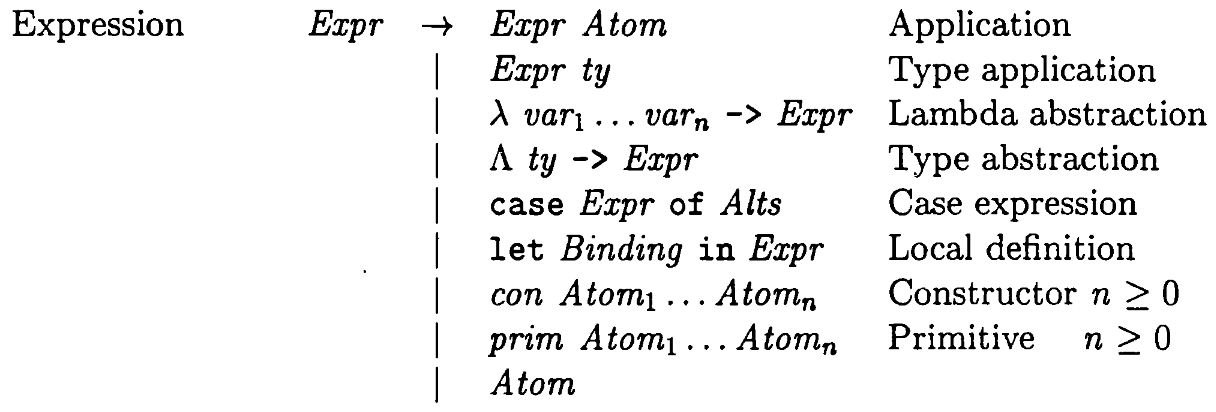
\includegraphics[width=1\textwidth]{pics/core.png}
\end{frame}
\begin{frame}
\frametitle{Syntaxe de Core}
$
\begin{array}{ccll}
\aTerm, \aTerm[1], \aTerm[2] & ::= & & \\
& | & \aBase & \text{(base)} \\
& | & \tfun \aVar \aType \aTerm & \text{(abstraction)} \\
& | & \tapp \aTerm \aBase & \text{(function application)} \\
& | & \tlet \aVar \aTerm {\aTerm[1]} & \text{(let binding)} \\
& | & \ite \aTerm {\aTerm[1]} {\aTerm[2]} & \text{(conditional)}\\
& | & \ttyfun \aTypeVar \aTerm & \text{(type abstraction)} \\
& | & \ttyapp \aTerm \aType & \text{(type application)} \\
& | & \ttyann \aTerm \aType & \text{(type annotation)}
\end{array}
$\\
$
\begin{array}{ccll}
\aBase & ::= & & \\
& | & \aVar & \text{(variable)} \\
& | & \true & \text{(true)} \\
& | & \false & \text{(false)} \\
\end{array}
$
$
\begin{array}{ccll}
\aType, \aType[1] & ::= & & \\
& | & \aTypeVar & \text{(type variable)} \\
& | & \tyBool & \text{(bool type)} \\
& | & \aDomType \to \aCodType & \text{(function type)} \\
& | & \tforall \aTypeVar \aType & \text{(polymorphic type)} \\
\end{array}
$
\end{frame}
\begin{frame}
\frametitle{Constant folding}
Règles
\begin{mathpar}
\begin{array}{cc}
\aRule   { }
         {\simplBeta {\tapp {(\tfun \aVar \aType \aTerm)} \aBase} {{\subs \aTerm {\envElem \aVar \aBase}}}}
         {}
&
         \aRule   { }
         {\simplBeta {{\ite \true \aTerm {\aTerm[1]}}} {\aTerm}}
         {}
\\
\aRule   { }
         {\simplBeta {\ttyapp {(\ttyfun \aTypeVar \aTerm)} \aType} {{\subs \aTerm {\envElem \aTypeVar \aType}}}}
         {}
&
\aRule   { }
         {\simplBeta {{\ite \false \aTerm {\aTerm[1]}}} {\aTerm[1]}}
         {}
\end{array}
\end{mathpar}
Exemple
\[\begin{aligned}[t]
&\ite {(\tapp {(\tfun \aVar \tyBool \aVar)} {\false})} {\aVar} {\aVar[1]} \\
&\rightsquigarrow \ite {\false} {\aVar} {\aVar[1]} \\
&\rightsquigarrow {\aVar[1]}
\end{aligned}\]
\end{frame}
\begin{frame}
\frametitle{Vue d’ensemble}
Structure du dépôt \\
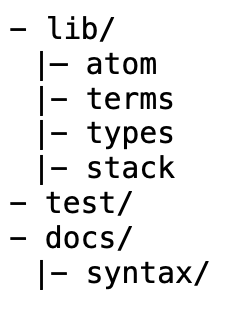
\includegraphics[scale=0.5]{pics/repo_structure.png} \\
Etapes de réalisation \\
\begin{itemize}
    \item Mise en place de la syntaxe, de l’alpha-renommage, et du typechecker (PR !1, !5, !6)
    \item Ajout des contextes d’évaluation (PR !4)
    \item Ajout de la simplification (PR !9)
    \item Preuve de correction (PR !10)
    \item Rectification du code grâce à la preuve (PR !11)
\end{itemize}
\end{frame}
\begin{frame}
\frametitle{Compétences techniques}
\begin{itemize}
    \item Construire une preuve en autonomie
    \item Programmation en OCaml
    \item Ecriture de LaTex avec des macros
    \item Utilisation professionnelle de git: code review, git flow
\end{itemize}
Répartition du travail équitable
\end{frame}
\begin{frame}
\frametitle{Principales difficultés}
\begin{itemize}
    \item Découverte de nouveaux outils en OCaml et LaTeX
    \item Utilisation raisonnée de git
    \item Nouveautés théoriques
    \item Schéma de preuve
\end{itemize}
\end{frame}
\begin{frame}
\frametitle{Algorithme: go}
$\begin{aligned}[t]
t = \ite{\tapp{(\tfun{\aVar}{\tyBool}{\aVar})}{\true}}{\ttyfun{\aTypeVar}{\aTerm[1]}}{\ttyfun{\aTypeVar}{\aTerm[2]}}
\end{aligned}$ \\
$\begin{aligned}[t]
&\go {\scoped {(\ttyapp{(\ttyfun{\aTypeVar[1]}{\ttyapp \aTerm {\aTypeVar[1]}})}{\tyBool}  )}{\envId}}{\emptyStack} \\
\pause
&=\go {\scoped {(\ttyfun{\aTypeVar[1]}{\ttyapp \aTerm {\aTypeVar[1]}})} {\envId}} {(\aPolyFrameAll {\tyBool} {\envId})} \\
\pause
&=\go {\scoped {(\ttyapp \aTerm {\aTypeVar[1]})} {\envElem {\aTypeVar[1]} \tyBool}} {\emptyStack} \\
\pause
&=\go {\scoped {\aTerm} {\envElem {\aTypeVar[1]} \tyBool}} {(\aPolyFrameAll {\aTypeVar[1]} {\envElem {\aTypeVar[1]} \tyBool})} \\
\pause
&=\go {\scoped {(\tapp{(\tfun{\aVar}{\tyBool}{\aVar})}{\true})} {\envElem {\aTypeVar[1]} \tyBool}} {\aStack}\\
& \text{avec } \aStack = \nonEmptyStack {\aIteFrameAll {\ttyfun{\aTypeVar}{\aTerm[1]}} {\ttyfun{\aTypeVar}{\aTerm[2]}} {\envElem {\aTypeVar[1]} \tyBool}} {\aPolyFrameAll {\aTypeVar[1]} {\envElem {\aTypeVar[1]} \tyBool}} \\
\pause
&=\go {\scoped {(\tfun{\aVar}{\tyBool}{\aVar})} {\envElem {\aTypeVar[1]} \tyBool}} {(\nonEmptyStack {\aFunFrameAll {\true} {\envElem {\aTypeVar[1]} \tyBool}} {\aStack})}\\
\pause
&=\go {\scoped {\aVar} {\envExtend {\envElem {\aTypeVar[1]} \tyBool} \aVar \true}} {\aStack}\\
\pause
&=\go {\scoped {(\ttyfun{\aTypeVar}{\aTerm[1]})} {\envElem {\aTypeVar[1]} \tyBool}} {(\aPolyFrameAll {\aTypeVar[1]} {\envElem {\aTypeVar[1]} \tyBool})} \\
\pause
&=\go {\scoped {\aTerm[1]} {\envExtend {\envElem {\aTypeVar[1]} \tyBool} \aTypeVar \tyBool}} {\emptyStack}\\
\end{aligned}$
\end{frame}
\begin{frame}
\frametitle{go: spécification complète}
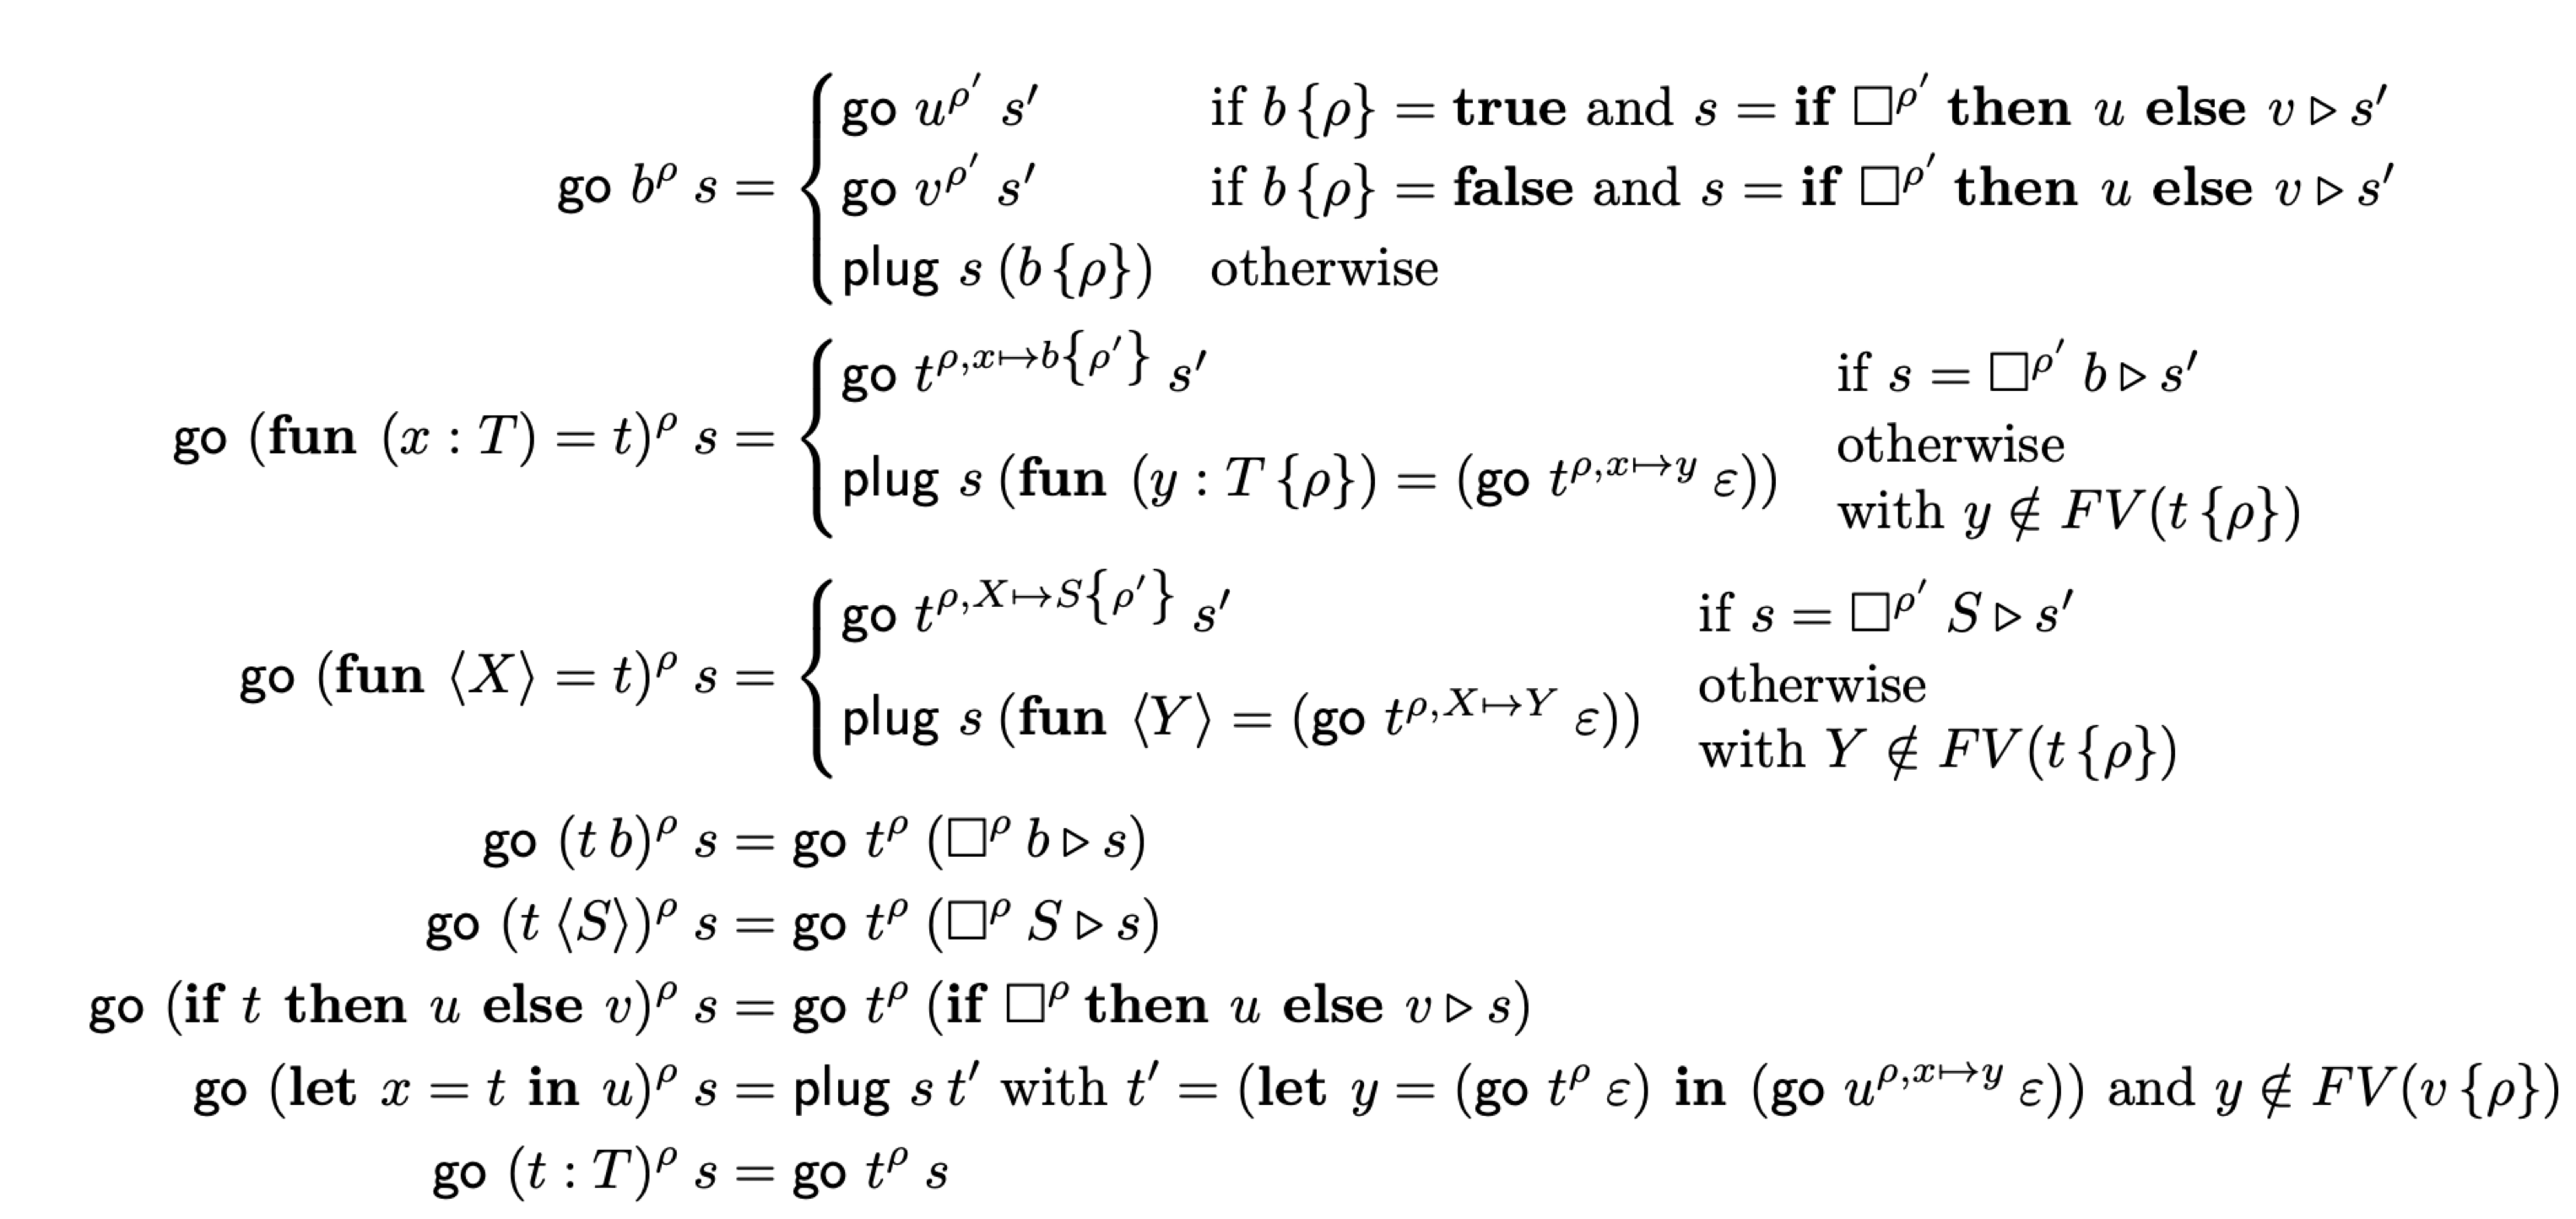
\includegraphics[scale=0.2]{pics/go_spec.png}
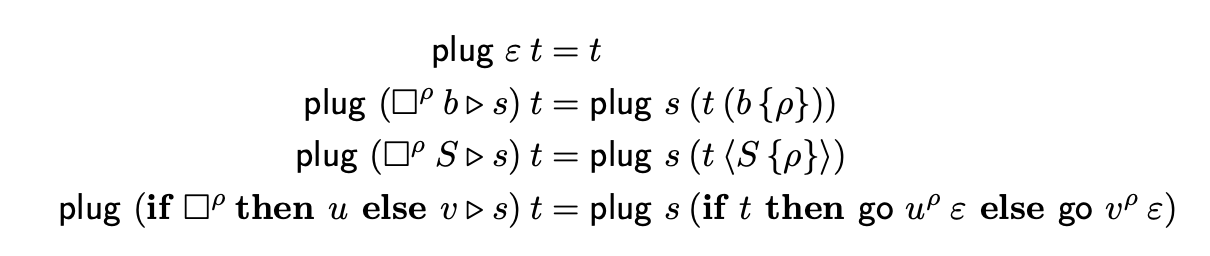
\includegraphics[scale=0.5]{pics/plug_spec.png}
\end{frame}
\begin{frame}
\frametitle{Testabilité}
\begin{itemize}
    \item 142 tests, qui s’exécutent en 0.019s
    \item La preuve a permis de corriger le code
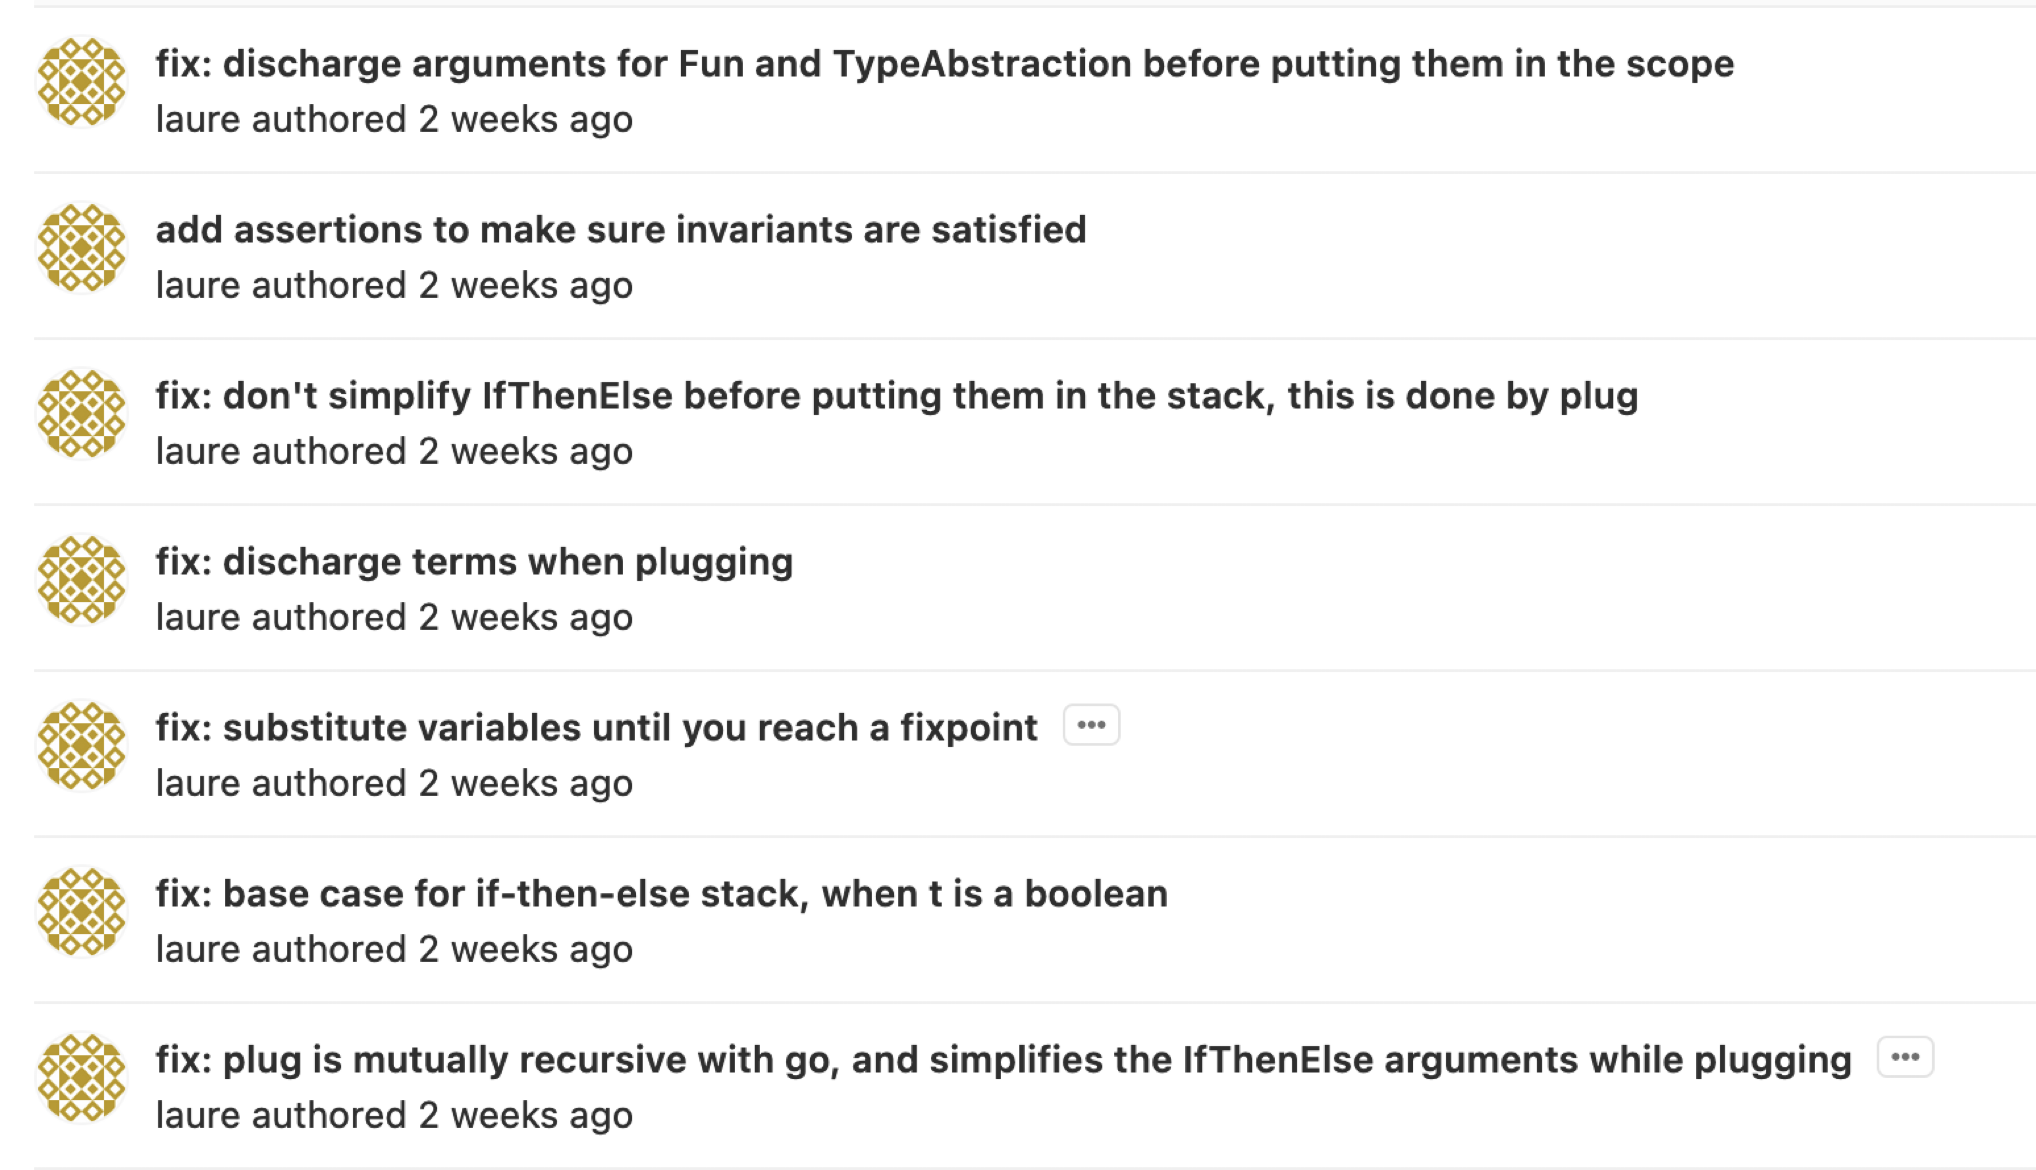
\includegraphics[scale=0.25]{pics/bug_fix_commits.png}
\end{itemize}
\end{frame}
\begin{frame}
\frametitle{Conclusion}
On a appris:
\begin{itemize}
    \item à bien programmer en OCaml
    \item à construire une preuve en autonomie
    \item à écrire un document conséquent en LaTeX
    \item à adapter nos objectifs
\end{itemize}
Une version 2.0:
\begin{itemize}
    \item avec une interface et un parser
    \item avec du let-floating et de l’inlining
    \item avec un outil de comparaison de performance
\end{itemize}
A changer:
\begin{itemize}
    \item commencer après le cours de semantique
    \item problème d’adéquation entre le problème et les objets qu’on a l’habitude de manipuler (preuve de programme)
    \item être plus strictes avec git pour éviter des gros conflits
\end{itemize}
\end{frame}
\end{document}
